% commandes pour compiler le rapport:
% dans le terminal, se placer dans le dossier contenant le fichier modele_rapport_latex.tex et compiler deux fois:
% linux:
% pdflatex modele_rapport_latex.tex -output-directory=output && pdflatex modele_rapport_latex.tex -output-directory=output && mv output/modele_rapport_latex.pdf ./
% windows:
% pdflatex modele_rapport_latex.tex -output-directory=output && pdflatex modele_rapport_latex.tex -output-directory=output && move -Y output\modele_rapport_latex.pdf .\
%
\documentclass[a4paper]{article} % Utilisation de la classe article
% Options possibles : 10pt, 11pt, 12pt (taille de la fonte)
%                     oneside, twoside (recto simple, recto-verso)
%                     draft, final (stade de développement)

\usepackage[utf8]{inputenc}  % LaTeX, comprends les accents !
\usepackage[T1]{fontenc}  % Police contenant les caractères français
\usepackage[french]{babel}  % Le document est en français
\usepackage{fullpage}  % pour les marges
\usepackage{graphicx}  % pour inclure des images

%\pagestyle{headings}  % Pour mettre des entêtes avec les titres
						% des sections en haut de page

\usepackage{datetime}  % pour la date
\newdate{frontpagedate}{12}{05}{2024}  % jour, mois, année

% \begin{center}               % pour centrer 
% 	\includegraphics[scale=1]{}   % insertion d'une image
% \end{center} % fichier contenant les packages et les commandes personnalisées


\begin{document}
\begin{titlepage}
\begin{center}
\vspace{2cm}
%\textsc{ Oregon State University}\\[1.5cm]

\includegraphics[width=0.4\textwidth]{root/UM1.png}~\\[1cm]
\vspace{2cm}

% Title
\hrule
\vspace{.5cm}
{\huge\bfseries{Hex-Ta(c)tique\\Projet de programmation 2}} % title of the report
\vspace{.5cm}

\hrule
\vspace{1.5cm}

\textsc{\textbf{Auteurs}}\\
\vspace{.5cm}
\centering

% add your name here
Al Ayoubi Ibrahim\\
Bigey Raphaël\\
Bonetti Timothée\\
Lejeune Ivan\\

\vspace{4cm}

\centering \displaydate{frontpagedate} % Dags dato
\end{center}
\end{titlepage}  % page de garde
\newpage


\tableofcontents  % Table des matières
\newpage


\section{Présentation du sujet}
% présenter le problème étudié et le contexte dans lequel il se positionne
Dans le cadre de notre projet de programmation de L3 Informatique, nous avons
choisi de travailler sur la résolution de jeux de stratégie combinatoire.
Nous avons choisi de nous intéresser à deux jeux de stratégie combinatoire en
particulier: le jeu du hex et le jeu de l'Awalé.

% motiver l'intérêt du problème étudié par rapport à votre parcours d'études
% et au monde de l'informatique
Ce projet est motivé par notre intérêt pour la théorie des jeux, et par notre 
désir de comprendre les mécanismes de résolution de jeux de stratégie 
combinatoire.
L'étude de ces jeux nous permettra de mieux comprendre les algorithmes de 
recherche et d'optimisation, et de nous familiariser avec les techniques de 
programmation avancée. A l'avenir, ces résultats pourront être utilisés dans
un cadre plus général pour la résolution de problèmes complexes, par exemple
pour les échecs ou le go.

% présenter les différentes approches possibles pour la résolution du problème
% et en particulier celle choisie
Il existe plusieurs approches possibles pour la résolution de jeux de stratégie
combinatoire. Parmi les approches les plus courantes, on trouve les algorithmes
de recherche en profondeur, les algorithmes de recherche de chemin, les
algorithmes de recherche de meilleure réponse, les algorithmes de Monte-Carlo,
les algorithmes de renforcement, etc.
Pour ce projet, nous avons choisi d'implémenter deux algorithmes en particulier
pour la résolution des jeux de hex et d'Awalé: l'algorithme Minimax avec élagage
alpha-bêta pour le jeu de hex, et l'algorithme de Dijsktra pour le jeu de l'Awalé.

Les principaux avantages de ces algorithmes sont les suivants:
\begin{itemize}
	\item L'algorithme Minimax avec élagage alpha-bêta est un algorithme de recherche
	qui permet de trouver la meilleure stratégie pour un joueur dans un jeu à deux
	joueurs. Cet algorithme est très efficace pour les jeux de stratégie combinatoire
	comme le hex, car il permet de réduire le nombre de nœuds explorés lors de la
	recherche de la meilleure stratégie.
	\item L'algorithme de Dijsktra est un algorithme de recherche de chemin qui permet
	de trouver le chemin le plus court entre deux nœuds dans un graphe. Cet algorithme
	est très efficace pour le jeu de l'Awalé, car il permet de trouver la meilleure
	stratégie pour un joueur en minimisant le nombre de graines capturées par l'adversaire.
\end{itemize}

% donner le cahier des charges détaillé :
Le cahier des charges détaillé est disponible en annexe.
A RAJOUTER\@: Le cahier des charges détaillé  % Présentation du sujet
\newpage


\section{Technologies utilisées}

% présenter les langages de programmation et les outils utilisés dans le cadre
% du projet
Pour la réalisation de ce projet, nous avons utilisé les langages de programmation suivants:
\begin{itemize}
	\item Python pour l'implémentation des algorithmes de résolution des jeux et la logique du jeu,
	\item HTML, CSS et JavaScript pour l'implémentation de l'interface graphique des jeux,
	\item UML pour la modélisation des classes et des cas d'utilisation,
	\item Git pour la gestion du code source et le suivi des versions,
	\item Visual Studio Code pour l'écriture du code et le débogage,
	\item GitHub pour l'hébergement du code source et la collaboration,
	\item LaTeX pour la rédaction du rapport,
	\item Draw.io pour la création des diagrammes UML
\end{itemize}

% justifier le choix et l'intérêt des langages utilisés  % Technologies utilisées
\newpage


\section{Développements Logiciel: Conception, Modélisation, Implémentation} 
\subsection{Description des modules utilisés}
% présenter les développements logiciels réalisés dans le cadre du projet
Pour la réalisation de ce projet, nous avons développé un logiciel qui permet de jouer
aux jeux de stratégie combinatoire abstraits du Hex et de l'Awalé. Ce logiciel est
composé de plusieurs modules, dont les principaux sont les suivants:

% présenter les principaux modules du logiciel développé dans le cadre du projet
% Utiliser le langage UML pour la modélisation : donner le diagramme de cas
% d'utilisation et le diagramme des classes
\begin{itemize}
    \item \textbf{Module Hex:} Ce module contient les classes et les fonctions nécessaires
    pour jouer au jeu de Hex. Il contient notamment la classe \texttt{HexBoard} qui 
    représente le plateau de jeu et les joueurs du jeu de Hex. Ce module contient également 
    les fonctions pour l'implémentation de l'algorithme Minimax avec élagage alpha-bêta pour 
    la résolution du jeu de Hex.
    
    \item \textbf{Module Awalé:} Ce module contient les classes et les fonctions nécessaires
    pour jouer au jeu de l'Awalé. Il contient la classe \texttt{AwaleBoard} qui représente le
    plateau de jeu et les joueurs du jeu de l'Awalé. Ce module contient également les fonctions
    pour l'implémentation de l'algorithme de Dijsktra pour la résolution du jeu de l'Awalé.
    
    \item \textbf{Module Interface Graphique:} Ce module contient les fichiers HTML, CSS et
    JavaScript nécessaires pour l'implémentation de l'interface graphique des jeux de Hex et
    d'Awalé. Il contient notamment les fichiers \texttt{home.html}, \texttt{hex.html} et
    \texttt{awale.html} qui permettent à l'utilisateur de choisir le jeu auquel il veut jouer
    et les paramètres de la partie. Il contient également des fichiers JavaScript pour la
    gestion des événements et des interactions avec l'utilisateur.
    
    \item \textbf{Module Tests:} Ce module contient les fichiers de tests unitaires pour les
    classes et les fonctions des modules Hex et Awalé. Il contient notamment les fichiers
    \texttt{test\_hex.py} et \texttt{test\_awale.py}, qui permettent de tester les classes
    et les fonctions des modules Hex et Awalé. ***TODO: Ajouter les tests unitaires***
\end{itemize}


% décrire les fonctionnalités de l'interface graphique implémentée (si votre 
% logiciel dispose d'une interface graphique)
\paragraph{Fonctionnalités de l'interface graphique}
L'interface graphique de notre logiciel comprend une page d'accueil qui permet à l'utilisateur
de choisir le jeu auquel il veut jouer (Hex ou Awalé), une page principale pour chaque jeu
qui permet à l'utilisateur de choisir les paramètres de la partie (taille du plateau (pour Hex),
mode de jeu (joueur contre joueur, joueur contre ordinateur, ordinateur contre ordinateur),
niveau de difficulté (pour l'ordinateur), etc.), et une page de jeu qui permet à l'utilisateur
de jouer au jeu choisi. L'interface graphique est implémentée en HTML, CSS et JavaScript, et
elle communique avec les modules Hex et Awalé via des appels de fonctions JavaScript à des
fonctions Python via des requêtes json et le module Flask.

% présenter les principales structures de données définies dans le cadre du
% projet. Décrire le format des données en entrée ou encore les conventions
% utilisées pour les entrées de vos programmes. Décrire les procédures de
% lecture et validation des entrées.
\paragraph{Structures de données}
Les principales structures de données définies dans le cadre de ce projet sont les classes
\texttt{HexBoard} et \texttt{AwaleBoard} qui représentent les plateaux de jeu du Hex et de
l'Awalé, respectivement. Ces classes contiennent les attributs et les méthodes nécessaires
pour représenter les plateaux de jeu et les joueurs, et pour effectuer les opérations de jeu
(placement de pions, déplacement de pions, etc.). Les données en entrée des programmes sont
sous forme de chaînes de caractères qui représentent les paramètres de la partie (taille du
plateau, mode de jeu, niveau de difficulté, etc.). Les procédures de lecture et de validation
des entrées sont effectuées par les fonctions des modules Hex et Awalé qui vérifient que les
paramètres de la partie sont valides avant de commencer la partie.

\subsection{Interaction entre fichiers}
% Explication de l'interaction entre les fichiers pendant une partie
Les fichiers de l'application interagissent entre eux de la même façon lors d'une partie de Hex ou 
d'Awalé. Le fichier \texttt{app.py} héberge l'application flask et gère l'interaction entre le frontend et le 
backend.

\paragraph{Initialisation de la partie}
La sélection du jeu et des paramètres de la partie se fait dans le fichier \texttt{home\_hex.html}
(respectivement \texttt{home\_awale.html} pour l'Awalé). Ces informations seront envoyées au fichier \texttt{app.py}
lors de l'appui sur l'un des boutons de lancement de partie. Le bouton sélectionné appellera dans le fichier \texttt{app.py} la 
fonction adéquate renvoyant la page html correspondant aux choix fait par le(s) joueur(s). En parallèle, une instance du plateau de
jeu désiré sera créée dans l'\texttt{app.py}. 

\paragraph{Déroulement d'une partie}
Lorsqu'une partie est jouée, l'information des pièces placées au Hex, ou des graines déplacées à l'Awalé est récupérée par
le fichier JavaScript adapté (par exemple \texttt{game\_hexia.js} si la partie est une partie de Hex joueur contre l'ordinateur, ou encore 
\texttt{game\_awale.js} si la partie est une partie d'Awalé joueur contre joueur). Cette information est gérée par le capteur d'événements
hex.onclick pour le Hex et pit.onclick pour l'Awalé. Si un tel événement est entendu, le fichier JavaScript correspondant envoie une requête 
json au fichier \texttt{app.py} afin de savoir si le coup est valide. La validité du coup est gérée par une fonction appelée dans la classe du
plateau de jeu adéquat. Si le coup est valide, alors celui-ci est joué et rajouté à l'instance du plateau de jeu, et est renvoyé au fichier 
JavaScript qui va s'occuper du nouvel affichage graphique (En modifiant le CSS ou le html). Si une erreur est attrapée, elle est renvoyée
au fichier JavaScript qu'il va gérer en affichant une alerte sur l'écran du joueur indiquant la non-validité du coup. Lors du placement de chaque
hex (déplacement de graines pour l'Awalé), la fonction \textit{check\_winner} de la classe du plateau est appelée afin de vérifier si un joueur à 
gagné. Si c'est le cas, alors la fonction questionnée par la requête json renvoie la variable \textsf{game\_over} égale à \textbf{True}. 
En récupérant cette variable, le fichier JavaScript va pouvoir procéder à une animation indiquant au(x) joueur(s) que la partie est terminée.







% Statistiques : nombre de modules/composantes/classes/scripts développés.
% Nombre de lignes de code.
\paragraph{Statistiques}
Voici quelques statistiques sur le logiciel développé dans le cadre de ce projet:
\begin{itemize}
    \item Nombre de modules (sans les tests): 39
    \item Nombre de classes : 11 (principalement dans les modules Hex et Awalé)
    \item Nombre de fonctions : 68 (en Python) et 99 (en JavaScript) pour 167 en tout
    \item Nombre de lignes de code : 1 405 (en Python), 2008 (en JavaScript), 553 (en HTML), 1 331 (en CSS)
    et 480 (en \LaTeX) pour un total de 5 777 lignes de code
\end{itemize}  % Développements Logiciel: Conception, Modélisation, Implémentation
\newpage


\section{Moteur de jeux combinatoires abstrait}


% présenter les principaux algorithmes utilisés comme moteur de jeu combinatoires absrtaits
%methode de monte carlo
%min max


% evaluer la complexité théorique en temps des algorithmes présentés.

Implémenter un algorithme pour jouer a des jeux combinatoires contre l'ordinateur est l'un des objectifs principaux du projet
Hex-Ta(c)tique mais alors une problématique apparait: Quels sont les algorithmes qui permettent a un ordinateur
de jouer a un jeu combinatoire abstrait quels sont leurs points forts et leurs inconvénients dans cette section nous allons
présenter 2 algorithmes principaux que sont: la Recherche arborescente Monte-Carlo (Monte carlo Three Search) et le
l'algorithme du min-max avec élagage alpha beta:

\subsection {la Recherche arborescente Monte-Carlo}

\paragraph {présentation}
la recherche arborescente Monte Carlo ou Monte Carlo tree search (MCTS) est un algorithme de recherche heuristique
Il est principalement utilisé dans le cadre de mis en place d'intelligence artificielle pour des jeux tels que les jeux combinatoires
comme le go mais pas uniquement en effet il est aussi utilisé pour les moteurs de jeux des échecs comme le moteur Alpha Zero 
l'un des leaders en terme d'intelligence de jeux aux échecs. Cet algorithme peut même être implémente dans des jeux ou le hasard 
apparait par exemple au poker.

\paragraph {MCTS - fonctionnement succinct}
Monte Carlo Three Seach ou MCTS est un algorithme qui explore l'arbre des possibles. La racine est la configuration initiale du jeu.
Chaque nœud est une configuration (une situation en jeu) et ses enfants sont les configurations suivantes. MCTS conserve en mémoire un arbre qui correspond aux nœuds déjà explorés de l'arbre des possibles. Une feuille de cet arbre est soit une configuration finale (donc un des joueur a gagné) soit
soit un nœud dont aucun enfant n'a encore été exploré. Dans chaque nœud, on stocke deux nombres : le nombre de simulations gagnantes, et le nombre total de simulations. 
A chaque itération MCTS va chercher la feuille la plus prometteuse, comprendre la suite de coups qui possède la meilleure heuristique
et ensuite depuis cette feuille créer grâce aux règles du jeu une nouvelle feuille au hasard dans le but d'atteindre une configuration finale.
Dans le cas ou on trouve une configuration gagnante pour un joueur on va incrémenter le nombre de simulations gagnantes pour les nœuds
correspondant au joueur dans les parents de la feuille que l'on vient de créer.
L'algorithme répète cette opération un certain nombre de fois avant de choisir un coup ie: choisir le coup qui a le plus de simulations
gagnantes et le moins de simulations totales.

%exemple.\dots


\subsection {algorithme MinMax}

\paragraph {présentation}
L'algorithme MinMax comme MCTS est un algorithme décisionnel mais celui ci s'applique sur des jeux a somme nulle: c'est a dire
un jeu où la somme des gains et des pertes de tous les joueurs est égale à 0. Cela signifie donc que le gain de l'un constitue 
obligatoirement une perte pour l'autre. L'algorithme va utiliser cette propriété dans sa recherche pour le meilleur coup possible.
En effet il amène l'ordinateur à passer en revue toutes les possibilités pour un nombre limité de coups et à leur assigner une valeur 
qui prend en compte les bénéfices pour le joueur et pour son adversaire. Le meilleur choix est alors celui qui minimise les pertes 
du joueur tout en supposant que l'adversaire cherche au contraire à les maximiser (d'où le nom MinMax)

\paragraph {MinMax - fonctionnement succinct}
Comme le MCTS le MinMax va explorer l'arbre des possibles. L'algo va explorer toutes les possibilités et mettre une valeur positive ou négative
a chaque feuille de l'arbre qui sont des nœuds terminaux ou des nœuds à la profondeur de recherche maximale Positive si la position favorise le joueur 
que joue l'ordinateur (le joueur maximisant) négative dans le cas contraire. Les nœuds non feuilles héritent de leur valeur a l'aide de leurs enfants.
Ainsi, les nœuds conduisant à un résultat favorable, comme une victoire, pour le joueur maximisant ont des scores plus élevés que les nœuds 
plus favorables pour le joueur minimisant. Les valeurs heuristiques pour les nœuds feuilles terminaux (fin du jeu) sont des scores correspondant 
à la victoire, à la défaite ou à l'égalité pour le joueur maximisant. Pour les nœuds feuilles non terminaux à la profondeur maximale de recherche, 
une fonction d'évaluation estime une valeur heuristique pour le nœud. La qualité de cette estimation et la profondeur de recherche déterminent la 
qualité et la précision du résultat final de minimax.

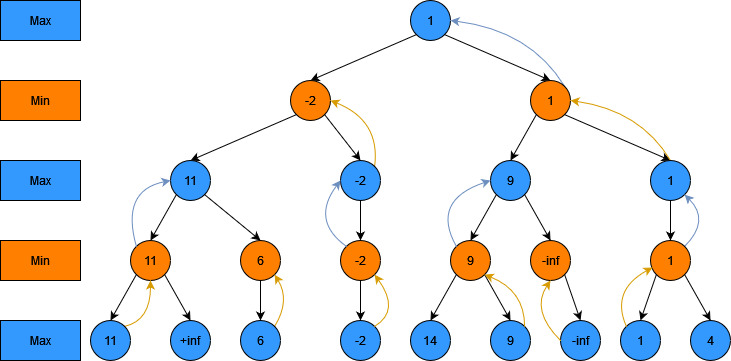
\includegraphics[width=0.4\textwidth]{root/MinMax.jpeg}~\\[1cm]  % Algorithmes et Analyse
\newpage


% illustrer les performances ainsi que l'efficacité du logiciel implémenté
% a l'aide de graphiques.


% analyser (et comparer, si plusieurs) les performances des solutions 
% implémentées


% présenter les bancs d'essais (ou les procédures utilisées pour la génération)
% des données) utilisés pour les tests du logiciel.

\section{Observations de l'algorithme MinMax sur nos jeux}
Une fois l'implémentation de l'algorithme \emph{MinMax} faite sur nos deux
jeux combinatoires, nous pouvons nous demander, est-ce que cet algorithme est adapté pour le jeu du Hex et de l'Awalé?
Nous observons que les performances du \emph{MinMax} sont très différentes d'un jeu à l'autre. Dans cette section nous étudierons ces différences.

\subsection{Hexgame: Performances décevantes}
L'algorithme \emph{MinMax} développé sur le jeu du Hex n'arrive quasiment jamais à battre un humain, et cela, pour
deux raisons principales: la faible profondeur, et la difficulté à trouver une fonction d'évaluation satisfaisante.

\subsubsection{Trop grande complexité} Le premier problème provient du nombre de coups possibles à chaque tour.
En effet, sur un plateau classique de dimension $13\times13$, le premier joueur a 169 coups possibles. Au coup suivant, il y en a 168 etc\dots Cela rend les calculs lents. 
Si l'ordinateur joue en premier, et que la profondeur de calcul est de 6, celui-ci doit calculer pas moins de $2.1298467e+13$ (soit $169\times168\times167\times166\times165\times164$)
fois la fonction d'évaluation. Cela n'est pas réalisable en temps réaliste. Dans notre implémentation, la taille des côtés du plateau varie entre
une longueur de 5 cases et de 17. Nous avons remarqué que pour un plateau de dimension $11\times11$, et une profondeur demandée de 4, l'algorithme
mettait déjà plusieurs secondes à calculer le meilleur coup. Notons que ces calculs ne prennent pas en compte l'élagage alpha-bêta
qui optimise significativement le \emph{MinMax}. Même si une portion des nœuds n'est pas évaluée, le calcul reste trop lent pour pouvoir demander une
profondeur plus intéressante de 6 ou de 8 par exemple.
On peut aussi noter que la performance de l'élagage alpha-bêta dépend de la qualité de la fonction d'évaluation, qui, comme nous allons
le voir, n'est pas assurée.

\subsubsection{Fonction d'évaluation: Un vrai casse-tête}
Le \emph{MinMax} n'arrivant pratiquement jamais à une feuille terminale, nous avons compris que la fonction
d'évaluation du Hex devait être performante et peu coûteuse en temps. Cependant, faire comprendre à l'ordinateur si une position est gagnante
ou non s'est révélé très difficile. En effet, le Hex est un jeu possédant de nombreuses stratégies, et relier toutes ces stratégies en une
seule fonction d'évaluation n'est pas chose aisée. Ainsi, nous avons rapidement cherché à faire comprendre à l'ordinateur
quelle stratégie adapter au fur et à mesure de la partie. Parmi elles, la stratégie de faire des ponts (voir la figure 3) nous a posé beaucoup de problèmes.
Un pont permet au joueur de s'assurer de pouvoir connecter deux pièces lors d'un prochain coup. En effet, si le joueur adversaire cherche à bloquer
l'une des deux cases, nous avons juste à ajouter notre jeton afin de créer un chemin entre ces deux pièces. Nous pouvons noter que lorsque la profondeur de
réflexion du \emph{MinMax} est grande, il arrive parfois à remarquer que créer un pont est le meilleur coup. Mais nous revenons au problème n°1: la complexité.
Voir la section sur les fonctions d'évaluations pour voir quelles idées nous avons essayé. Notre fonction finale est capable de battre des humains sur de petits 
plateaux. Mais en général, lorsque le plateau est de grande dimension, la fonction d'évaluation prend de nombreuses secondes, voire minutes avant de jouer.

\begin{figure}[h]
    \begin{center}
        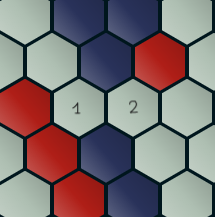
\includegraphics[scale=0.5]{root/pont.png}
    \end{center}
    \caption[1]{Ici bleu a créé un pont\footnotemark.}\label{fig:pont_bleu}
\end{figure}

\footnotetext{Si rouge joue sur la case 1, bleu joue sur la case 2, et relie ainsi les deux jetons bleus (respectivement si rouge joue sur la case 2)}



\subsection{Awalé: Bonnes performances}
\subsubsection{Une fonction d'évaluation efficace} 
Le jeu de l'Awalé possède un avantage significatif par rapport au Hex. En effet, le nombre maximum de coups
possible pour un joueur est de 6. Ainsi, l'arbre de recherche est bien plus petit que celui du Hex. L'algorithme \emph{MinMax} est donc efficace en termes de
temps et de performances avec une grande profondeur (la profondeur initiale est de 6 ou 8).

Le choix de notre fonction d'évaluation est arrivé naturellement pendant nos recherches. Nous avons implémenté la simple fonction cherchant à
maximiser les points de l'ordinateur tout en minimisant les points de son adversaire. Cette fonction combinée à une profondeur de taille 6 en fait un
adversaire redoutable que peu d'humains ont réussi à battre.

\subsection{Conclusion sur les performances du MinMax}
\emph{MinMax} est donc un algorithme capable d'être efficace lorsque le nombre de nœuds est petit à chaque itération. On peut alors
lui mettre une profondeur relativement grande afin d'explorer toutes les branches de cet arbre.
Cependant, lorsque le nombre de nœuds devient gigantesque, comme dans le Hex, l'algorithme ne devient plus très bon. Il est en effet très lent et peu performant.
Dans la bibliographie est disponible un lien vers un papier scientifique cherchant une bonne fonction d'évaluation pour le Hex.
Dans celui-ci, il est écrit que les ordinateurs battent les humains pour des petits plateaux, font jeu égal pour le plateau $9\times9$ mais
sont moins bons qu'un humain pour un plus grand plateau. On y voit aussi la difficulté de trouver une bonne fonction d'évaluation.
  % Analyse des résultats
\newpage

\include{./sources/10_strategie_gagnante} % strategie gagnante hexgame


\section{Gestion du Projet}

% présenter la gestion du projet et les documents de planification éventuellement
% rédigés (par exemple, le diagramme de Gantt).


% discuter les changements majeurs effectués en cours de projet  % Gestion du projet
\newpage


\section{Bilan et Conclusions}

% indiquer les fonctionnalités mise en oeuvre par rapport au cahier des charges
% de départ, les points ouverts et les perspectives pour le projet.
Nous avons implémenté la plupart des fonctionnalités prévues dans le cahier des charges, à l'exception de quelques
fonctionnalités mineures. Nous avons également ajouté des fonctionnalités supplémentaires qui n'étaient pas prévues
dans le cahier des charges, mais qui ont été jugées nécessaires pour améliorer la qualité du projet.

En bref, nous avons implémenté les fonctionnalités suivantes :

\begin{itemize}
    \item Possibilité pour les utilisateurs de jouer en JcJ au \emph{Hex} et à l'\emph{Awale}
    \item Possibilité pour les utilisateurs de jouer au JcIA au \emph{Hex} et à l'\emph{Awale}
    \item Possibilité pour les utilisateurs de regarder deux IA jouer au \emph{Hex} et à l'\emph{Awale}
    \item Possibilité pour les utilisateurs de changer de thème de couleur pour le jeu du \emph{Hex}
    \item Possibilité pour les utilisateurs de défaire un coup dans tous les modes de jeu (sauf IAvIA), pour le \emph{Hex} et l'\emph{Awale}
    \item Possibilité pour les utilisateurs de rejouer une partie dans tous les modes de jeu (sauf IAvIA), pour le \emph{Hex} et l'\emph{Awale}
    \item Possibilité pour les utilisateurs de choisir la taille du plateau de jeu pour le \emph{Hex}
    \item Possibilité pour les utilisateurs de choisir son camp (en JcIA) pour le \emph{Hex} et l'\emph{Awale}
    \item Possibilité pour les développeurs de tester, déployer et maintenir facilement l'application
    \item Possibilité pour les développeurs de rajouter facilement de nouvelles fonctionnalités
    \item Possibilité pour les développeurs de rajouter facilement de nouveaux jeux
\end{itemize}  % Bilan et Conclusions
\newpage

\section{Bibliographie}

% indiquer les ressources bibliographiques utilisées pour le projet


% donner des références exactes des travaux cités dans le texte permettant de
% trouver les articles ou livres cités en bibliothèque ou sur internet.

\sloppy
\begin{tabular}{|l|p{0.7\textwidth}|}
    \hline
    \textbf{Title} & \textbf{URLs} \\
    \hline
    Hex & 
    \begin{itemize}
        \item \href{https://www.pedagogie1d.ac-nantes.fr/medias/fichier/regles-jeu-de-hex_1465481131499-pdf?ID_FICHE=434770&INLINE=FALSE}{\url{https://www.pedagogie1d.ac-nantes.fr/medias/fichier/regles-jeu-de-hex_1465481131499-pdf?ID_FICHE=434770&INLINE=FALSE}}
        \item \href{http://www.cs.cornell.edu/~adith/docs/y_hex.pdf}{\url{http://www.cs.cornell.edu/~adith/docs/y_hex.pdf}}
        \item \href{https://en.wikipedia.org/wiki/Hex_(board_game)}{\url{https://en.wikipedia.org/wiki/Hex_(board_game)}}
        \item \href{https://gsurma.medium.com/hex-creating-intelligent-opponents-with-minimax-driven-ai-part-1-α-β-pruning-cc1df850e5bd}{Link to Article}
        \item \href{https://gsurma.medium.com/hex-creating-intelligent-adversaries-part-2-heuristics-dijkstras-algorithm-597e4dcacf93}{Link to Article}
        \item \href{https://www.labri.fr/perso/renault/working/teaching/projets/2019-20-S6-C-Hex.php}{\url{https://www.labri.fr/perso/renault/working/teaching/projets/2019-20-S6-C-Hex.php}}
        \item \href{https://www.lamsade.dauphine.fr/~cazenave/papers/hex-ria.pdf}{\url{https://www.lamsade.dauphine.fr/~cazenave/papers/hex-ria.pdf}}
        \item \href{https://hal.science/hal-02328750/document}{\url{https://hal.science/hal-02328750/document}}
    \end{itemize} \\
    \hline
    Stratégie gagnante & 
    \begin{itemize}
        \item \href{https://math.univ-lyon1.fr/irem/IMG/pdf/Hex.pdf}{\url{https://math.univ-lyon1.fr/irem/IMG/pdf/Hex.pdf}}
        \item \href{https://en.wikipedia.org/wiki/Hex_(board_game)}{\url{https://en.wikipedia.org/wiki/Hex_(board_game)}}
        \item \href{https://en.wikipedia.org/wiki/Zermelo's_theorem_(game_theory)}{\url{https://en.wikipedia.org/wiki/Zermelo's_theorem_(game_theory)}}
        \item \href{https://en.wikipedia.org/wiki/Game_complexity}{\url{https://en.wikipedia.org/wiki/Game_complexity}}
    \end{itemize} \\
    \hline
    Awalé & 
    \begin{itemize}
        \item \href{https://fondem.ong/awale-regles-du-jeu/}{\url{https://fondem.ong/awale-regles-du-jeu/}}
        \item \href{https://www.myriad-online.com/resources/docs/awale/francais/strategy.htm}{\url{https://www.myriad-online.com/resources/docs/awale/francais/strategy.htm}}
        \item \href{https://en.wikipedia.org/wiki/Awale}{\url{https://en.wikipedia.org/wiki/Awale}}
        \item \href{https://medium.com/@mol02office/implémentation-dune-ia-pour-l-awalé-partie-1-b298328d5e14}{Link to Article}
    \end{itemize} \\
    \hline
    Minimax &
    \begin{itemize}
        \item \href{https://en.wikipedia.org/wiki/Minimax}{\url{https://en.wikipedia.org/wiki/Minimax}}
        \item \href{https://en.wikipedia.org/wiki/Alpha–beta_pruning}{\url{https://en.wikipedia.org/wiki/Alpha–beta_pruning}}
        \item \href{https://fr.wikipedia.org/wiki/Élagage_alpha-bêta}{\url{https://fr.wikipedia.org/wiki/Élagage_alpha-bêta}}
    \end{itemize} \\
    \hline
\end{tabular}  % Bibliographie
\newpage

\section{Annexes}
% par exemple: fragments de code, manuel d'utilisation du logiciel etc


% \begin{thebibliography}{9}
% \bibitem{texbook}
% Donald E. Knuth (1986) \emph{The \TeX{} Book}, Addison-Wesley Professional.

% \bibitem{lamport94}
% Leslie Lamport (1994) \emph{\LaTeX: a document preparation system}, Addison
% Wesley, Massachusetts, 2nd ed.
% \end{thebibliography}
\vspace{0.3cm}
\subsection{Annexe I : Cahier des charges}
\vspace{0.3cm}
\subsubsection*{Objectifs du projet:}
Pour répondre aux attentes de notre projet, nous avons décidé de développer une application web sur laquelle 
nous pourrions jouer au jeu du Hex et de l'Awalé.

Pour chaque jeu nous devons implémenter les règles officielles afin d'assurer une cohérence
entre tous les joueurs. De plus, nous voulons fournir une interface graphique agréable pour l'utilisateur. 
Cela comprend donc une page d'accueil intuitive ainsi que des plateaux de jeu faciles d'utilisation.

\subsubsection*{Description des jeux:}
\begin{itemize}
    \item Hex:
    
    Le Hex est un jeu de stratégie à deux joueurs. Il se compose d'un plateau, de pions bleus
    et de pions rouges. Le plateau du jeu de Hex est composé de cases hexagonales formant un losange. La taille
    du plateau peut varier, mais est généralement de $11\times 11$. Deux côtés opposés du losange sont bleus, les deux 
    autres sont rouges. 

    Le joueur bleu commence. Les joueurs jouent chacun à leur tour. A chaque tour, un joueur place un pion de sa couleur sur une 
    case libre du plateau. Le premier joueur qui réussit à relier ses deux bords par un chemin de pions contigus de sa couleur
    a gagné. Il ne peut y avoir qu'un pion par case. Les pions posés le sont définitivement, ils ne peuvent être ni retirés, ni
    déplacés.\\
    \begin{figure}[h]
        \begin{center}
            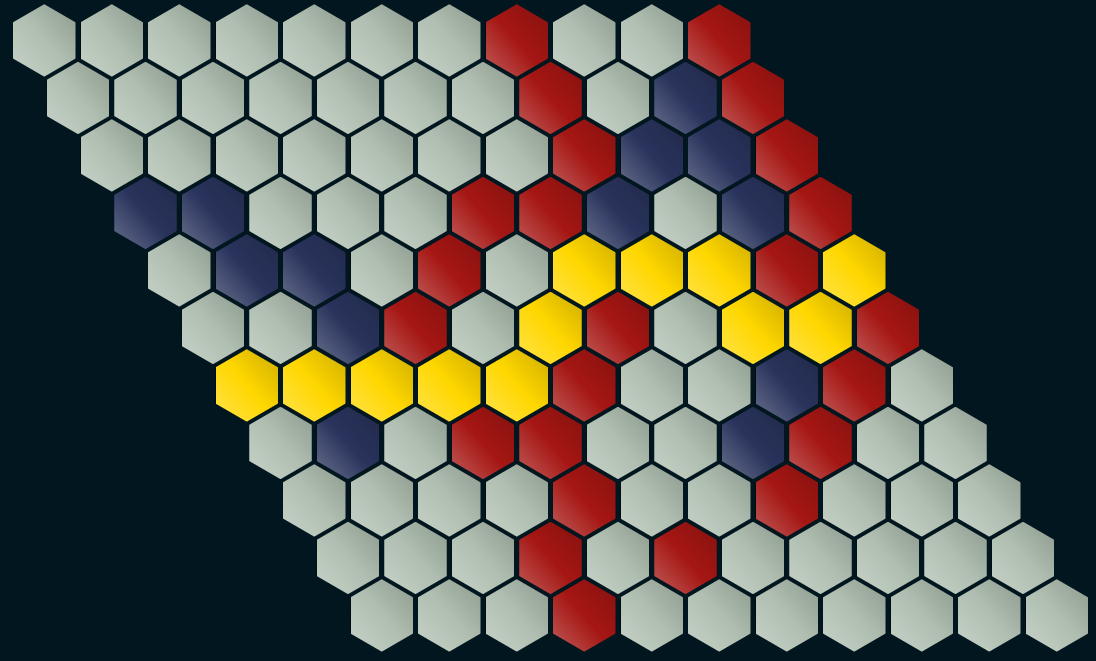
\includegraphics[scale=0.5]{root/hex_jeu_bleu}
        \end{center}
        \caption{Ici bleu a gagné, en reliant ses deux bords.}\label{fig:hex_jeu_bleu}
    \end{figure}
    

    \item Awalé:
    
    L'Awalé est un jeu de stratégie à deux joueurs. Il se compose d'un plateau et de graines. Au début de la partie, 4 graines se 
    situent dans chaque cases du plateau. Les joueurs jouent à tour de rôle. A chaque tour, le joueur prend toutes les graines d’un 
    des trous de son camp puis il les égrène une par une dans toutes les cases qui suivent sur sa rangée puis sur celle de son adversaire 
    suivant le sens de rotation (une graine dans chaque trou après celui où il a récupéré les graines).

    Le joueur « capture » des graines lorsque la dernière case où il pose une graine est une case du camp adversaire et si contient 2 ou 3 
    graines en comptant la nouvelle (elle contenait 1 ou 2 graines avant). Le joueur prend alors les graines de cette case (2 ou 3), puis il 
    prend également les graines de la case précédente si celle-ci répond aux mêmes conditions : être une case du camp adverse et contenir 2 ou 3 graines. 
    Il continue ainsi à prendre les graines des cases antérieures tant que celles-ci répondent aux conditions.

    La première façon qu'une s'achève est lorsqu’un joueur n’a plus de graines dans son camp alors que c’est à lui de jouer et que son adversaire n’est plus en mesure 
    de lui en apporter une selon la règle de « l’obligation de nourrir l’adversaire ». Dans ce cas, son adversaire gagne toutes les graines restantes. C’est 
    la fin par famine.

    La deuxième façon qu'une partie s'achève est lorsqu’il reste trop peu de graines pour qu’aucune prise ne soit désormais possible (en pratique 2 ou 3). 
    Chaque joueur récupère la ou les graines restantes de son camp. C’est la fin par indétermination.
    

\end{itemize}

\subsection*{Fonctionnalités de l'application:}
\begin{itemize}
    \item Possibilité de jouer en joueur contre joueur sur les deux jeux.
    \item Possibilité de jouer en joueur contre IA avec la couleur de notre choix sur  les deux jeux.
    \item Possibilité d'observer une partie entre deux IA sur les deux jeux.
    \item Possibilité d'annuler son dernier coup sur les deux jeux.
    \item Choisir la taille du plateau du Hex. 
    \item Divers boutons pour naviguer à travers l'application.
    \item Possibilité de réinitialiser le plateau des deux jeux lorsqu'on le souhaite.
\end{itemize}

\subsection*{Interface utilisateur:}
L'application s'ouvrira sur une page d'accueil sur laquelle nous pourrons choisir le jeu auquel nous souhaitons jouer.
Pour chaque jeu nous pourrons trouver une page home nous permettant de selectionner le mode de jeu que nous voulons
choisir. Nous retrouverons alors pour les deux jeux les modes joueur contre joueur, joueur contre IA et IA contre IA.

De nombreux boutons de couleur bleus seront mis en place afin de naviguer entre toutes les pages de l'application. D'autres
boutons plus petit seront disponibles. Ils permettront pendant les diverses parties de réinitialiser le plateau de jeu, ou de défaire 
notre dernier coup dans les modes de jeu joueur contre joueur et joueur contre IA.  % Annexes
\newpage

\subsection{HexGame et stratégie gagnante}

Au Hex, pour toutes les tailles de plateaux il existe une stratégie gagnante théorique pour le joueur qui commence.
Cependant, celle-ci n'est pas connue pour la plupart des tailles de plateaux. En effet, celle-ci demande une connaissance totale de toutes 
les parties possibles, ce qui n'est pas calculable en temps réaliste.

\subsubsection{Stratégies gagnantes et arbre du jeu}
Modélisons le jeu du Hex à l'aide d'un arbre représentant toutes les parties possibles. L'arbre commence avec la position 
initiale, un plateau vide. De cette racine partent autant de branches qu'il n'y a de possibilités pour 
le premier coup du premier joueur. On réitère cette action pour chaque nœud jusqu'à tomber sur des positions gagnantes pour l'un des deux joueurs.
%faire exemple
\begin{figure}[!htb]
    \begin{center}
        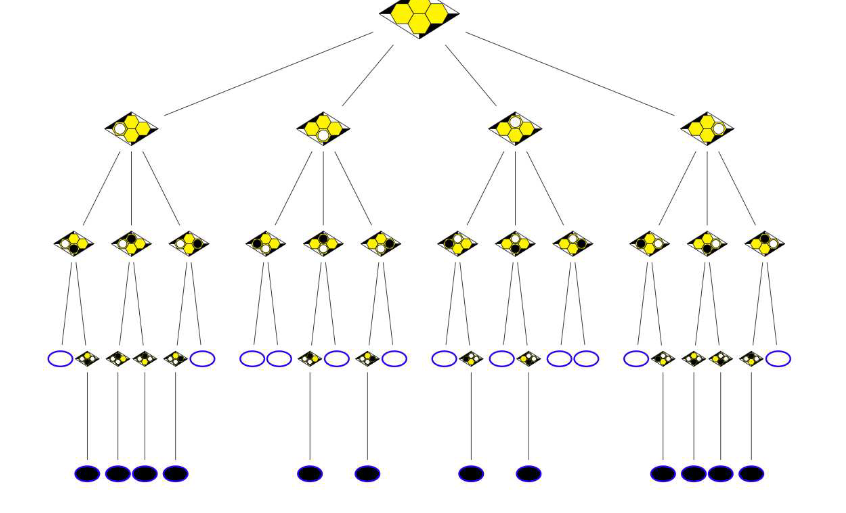
\includegraphics[width=0.4\textwidth]{root/strategie_gagnante.png}
    \end{center}
    \caption{Exemple pour un plateau $2\times2$}\label{fig:strategie_gagnante}
\end{figure}

L'arbre va nous aider à nous convaincre qu'il y a bien une stratégie gagnante pour l'un des deux joueurs. 
Le principe consiste à colorier tous les nœuds de l'arbre en blanc ou en noir, chaque
nœud colorié correspondant à une position à partir de laquelle le joueur de la couleur correspondante
possède une stratégie gagnante. 
Nous commençons par colorier en blanc les feuilles représentant une fin de
partie gagnée par les blancs, et en noir celles correspondant à la victoire du joueur noir.
Le reste du coloriage se fait progressivement. À un moment donné, on veut attribuer une couleur
à un nœud qui n'en a pas encore, mais dont toutes les branches descendantes mènent à des nœuds
déjà coloriés. Supposons que ce nœud représente une position à partir de laquelle c'est aux blancs de
jouer. Si au moins l'une des branches issues du nœud mène à un nœud blanc, alors on colorie le nœud
en blanc. Dans le cas contraire, c'est-à-dire si toutes les branches mènent à des nœuds coloriés en
noir, on le colorie en noir. On procède de façon symétrique si c'est aux noirs de jouer.
De cette manière nous sommes assurés de remplir l'arbre de nos couleurs jusqu'à la racine. 
Ainsi, la racine possède une stratégie gagnante.


\subsubsection{Remarques}
\begin{itemize}
    \item On voit que pour un plateau de dimension $2\times2$, l'arbre de tous les possibles possède déjà 24 feuilles et 52 branches.
    Il est calculé que pour un plateau de taille $11\times11$, le nombre de feuilles de l'arbre est
    approximativement $10^{98}$, et le nombre de positions totales que peut prendre le jeu est de $2.4\times10^{56}$.
    Donc en pratique, utiliser cette technique pour trouver la stratégie gagnante n'est pas possible.
    \item Il est aussi possible d'appliquer ce genre de raisonnement à d'autres jeux combinatoires abstraits pour essayer de
    prouver l'existence d'une éventuelle stratégie gagnante.
    \item Enfin, on remarque que cette façon de faire ressemble à l'algorithme MinMax s'il avait une profondeur de recherche
    infinie.
\end{itemize}

\subsubsection{Le premier joueur gagne à tous les coups}
On a vu qu'il existe une stratégie gagnante, mais on ne sait pas pour quel joueur est le gagnant. Dans ce paragraphe nous allons
prouver que le joueur 1, s'il joue parfaitement, gagne à tous les coups.

Puisque les matchs nuls sont impossibles, nous pouvons conclure que soit le premier, soit le deuxième joueur possède une stratégie
gagnante. Supposons maintenant que le deuxième joueur ait une stratégie gagnante.

Le premier joueur adopte alors la stratégie suivante: il effectue un mouvement arbitraire. Ensuite, 
il joue en utilisant la supposée stratégie gagnante du deuxième joueur mentionnée ci-dessus. Si,
en jouant cette stratégie, il doit jouer sur la case où un mouvement arbitraire a été fait, il effectue
un autre mouvement arbitraire. De cette manière, il suit la stratégie gagnante tout en ayant toujours une pièce
supplémentaire sur le plateau.

Cette pièce supplémentaire ne peut pas interférer avec l'imitation par le premier joueur de la stratégie gagnante.
En effet, une pièce supplémentaire pour le joueur 1 n'est jamais un désavantage. Par conséquent, le premier joueur peut
gagner.

Comme nous avons maintenant contredit notre hypothèse selon laquelle le deuxième joueur aurait une stratégie gagnante,
nous concluons qu'il n'y a pas de stratégie gagnante pour le deuxième joueur.

Par conséquent, il existe une stratégie gagnante pour le premier joueur.  % Stratégie gagnante au Hex
\newpage


\end{document}

